\documentclass{memoir}

\chapterstyle{hangnum}


\setcounter{secnumdepth}{2}


\usepackage{epigraph}
\usepackage{polyglossia}

\setmainlanguage[babelshorthands=true]{russian}    % Язык по-умолчанию русский с поддержкой приятных команд пакета babel
\setotherlanguage{english}                         % Дополнительный язык = английский (в американской вариации по-умолчанию)

%\setdefaultlanguage{russian}
%\setmainfont{CMU Serif}

%\setmonofont{Courier New}                          % моноширинный шрифт
%\newfontfamily\cyrillicfonttt{Courier New}         % моноширинный шрифт для кириллицы
%\defaultfontfeatures{Ligatures=TeX}                % стандартные лигатуры TeX, замены нескольких дефисов на тире и т. п. Настройки моноширинного шрифта должны идти до этой строки, чтобы при врезках кода программ в коде не применялись лигатуры и замены дефисов
%\setmainfont{Times New Roman}                      % Шрифт с засечками
%\newfontfamily\cyrillicfont{Times New Roman}       % Шрифт с засечками для кириллицы
%\setsansfont{Arial}                                % Шрифт без засечек
%\newfontfamily\cyrillicfontsf{Arial}               % Шрифт без засечек для кириллицы

\setmonofont{LiberationMono}[Scale=0.87]            % моноширинный шрифт
\newfontfamily\cyrillicfonttt{LiberationMono}[Scale=0.87]   % моноширинный шрифт для кириллицы
    
\defaultfontfeatures{Ligatures=TeX}                % стандартные лигатуры TeX, замены нескольких дефисов на тире и т. п. Настройки моноширинного шрифта должны идти до этой строки, чтобы при врезках кода программ в коде не применялись лигатуры и замены дефисов
\setmainfont{LiberationSerif}                      % Шрифт с засечками
%\setmainfont{CMU Serif}
\newfontfamily\cyrillicfont{LiberationSerif}       % Шрифт с засечками для кириллицы
\setsansfont{LiberationSans}                       % Шрифт без засечек
\newfontfamily\cyrillicfontsf{LiberationSans}      % Шрифт без засечек для кириллицы


\usepackage{amsthm}
\usepackage{url} 
\usepackage{hyperref} 


\usepackage[table]{xcolor}
%\let\newfloat\undefined
%\usepackage{floatrow}

% графика
\usepackage{graphicx}
\usepackage{tikz}                   % Продвинутый пакет векторной графики
\usepackage{pgfplots}
\pgfplotsset{compat=newest}
\usepackage{pgfplotstable}

\usepackage{wrapfig}

\usepackage{physics}
\usepackage{amsmath}
\usepackage{tikz}
\usepackage{mathdots}
\usepackage{yhmath}
\usepackage{cancel}
\usepackage{color}
\usepackage{siunitx}
\usepackage{array}
\usepackage{multirow}
\usepackage{amssymb}
\usepackage{gensymb}
\usepackage{tabularx}
\usepackage{booktabs}
\usetikzlibrary{fadings}
\usetikzlibrary{patterns}
\usetikzlibrary{shadows.blur}
\usetikzlibrary{shapes}




\begin{document}

\title{«Исследование скважин и пластов». Учебное пособие  Часть 1. Введение в исследование скважин и пластов. Промысловые и технологические исследования}
%\title{«Применение базовых алгоритмов анализа исследований нефтяных скважин»}
%\title{}

\maketitle

\tableofcontents{}
\chapter{Введение}

\section{Цели и задачи дисциплины}
Учебное пособие подготовлено в рамках курса "Исследования скважин и пластов", читаемого для студентов 4 курса РГУ нефти и газа (НИУ) имени И.М.Губкина и соответствует учебной программе курса по состоянию на 2020 год. 

Пособие описывает некоторые базовые подходы к построению и использованию математических моделей скважин и пластов, широко используемые при проведении и интерпретации исследований с использованием компьютеризированных алгоритмов. Рассматривается широкий диапазон исследований промысловых исследований - от технологических замеров ключевых параметров до внутрискважинных промысловых исследований и исследований пласта и призабойной зоны (во второй части). При этом акцент сделан именно на математических моделях и их реализациях в виде программных алгоритмов, что позволяет получить навыки построения моделей и интерпретации результатов исследований необходимые при широком использовании цифровых технологий в нефтедобычи. В работе широко используются открытые инструменты для проведения инженерных расчетов, что позволяет работать над решением задач на современном уровне без необходимости получения лицензий для коммерческих программ. 

Учебное пособие содержит набор задач, предназначенных для помощи в освоении дисциплины "Исследования скважин и пластов". Авторы уверены, что решение задач - лучший метод для изучения инженерных дисциплин. Поэтому в пособии сделан акцент именно на задачах. Теоретический материал приводится в минимальном виде, необходимом для решения задач. Для более подробного разбора теории приводятся ссылки на соответствующие материалы и статьи. Разобраны базовые примеры решения задач и приведены задачи для самостоятельной проработки в ходе семинаров. 

Пособие предназначено для студентов изучающих вопросы разработки и эксплуатации нефтяных и газовых месторождений, моделирование систем нефтедобычи, а также может быть полезным широкому кругу специалистов применяющих компьютерные математические модели нефтедобычи в практической деятельности. 

Учебное пособие является частью учебно методического комплекса для изучения дисциплины "Исследования скважин и пластов". Часть материалов комплекса доступна в сети интернет на общедоступных ресурсах. Это такие материалы как - программы и макросы для проведения инженерных расчетов, исходные данные для выполнения ряда заданий, видеоролики со вспомогательными материалами. Ссылки на ресурсы приводятся в пособии в состоянии актуальном на момент создания (предприняты все меры, чтобы обеспечить доступность ссылок на максимально длительный период, однако авторы не могут гарантировать работоспособность этих ссылок в длительной перспективе).




\section{Подход к изучению дисциплины Исследования скважин и пластов}
Курс "Исследования скважин и пластов" предназначен для того, чтобы дать студентам представление о современных подходах к проведению исследований на нефтяных месторождениях, а также о методах интерпретации их результатов. Рассматриваются различных виды исследований проводимых на скважинах введенных в эксплуатацию от технологических замеров и промысловых геофизических исследований до гидродинамических исследований.

Технологии проведения исследований и оборудование для их проведения с одной стороны достаточно хорошо описано в классической литературе и в интернет источниках, с другой стороны постоянно эволюционирует и меняется - появляются новые приборы и методы интерпретации, как правило использующие последние достижении техники и компьютерные технологии для интерпретации результатов. Остаются неизменными только физические принципы заложенные в основу исследований и методов их анализа. Понимая это авторы не гонятся за исчерпывающим описанием технологий и оборудования для проведения исследований. Вместо этого пособие описывает базовые принципы различных видов исследований выраженные в виде математических моделей. Причем рассматриваются компьютерные реализации этих моделей, которые могут быть использованы студентами и специалистами для обучения и для решения практических задач. Такие компьютерные модели лежат в основе большинства коммерческих программных комплексов, которые получили распространение в нефтяной промышленности, поэтому понимание основ их работы, сильных и слабых сторон, а также получение навыков построения компьютерных алгоритмов является залогом успешного и эффективного проведения исследования по глубокому убеждению авторов.

Большой объем материала и необходимость скорейшего создания учебного пособия заставили автором разбить пособие на две части. Часть 1 посвящена в большей степени исследованиям скважин - технологическим замерам (замеры дебита) и основам промысловых геофизических исследований (барометрия, термометрия и другие).  Часть 2 посвящена исследованию свойств пласта - гидродинамическим исследованиям скважин и построению простых моделей пласта и скважин - "прокси" моделям. При этом в этой части активно используют и модели скважин, разобранные в части 1.

В пособии рассматриваются принципы проведения и интерпретации распространенных видов исследований, которые лежат в основе многих расчетных методик. Понимание этих принципов и владение навыками проведения расчетов с использованием современных подходов позволит студенту решать широкий круг задач возникающих перед инженерами разработчиками на практике, а также облегчит самостоятельный разбор особенностей отдельных технологий. После разбора задач курса студенты смогут самостоятельно создать простые компьютерные алгоритмы для интерпретации базовых исследований скважин и пластов и при необходимости смогут развить их для обработки больших объемов данных по исследованиям и/или интерпретации нестандартных видов исследований. 

Из за широкого применения компьютерных алгоритмов в пособии читателю (и слушателю курсов) потребуется проявить навыки создания компьютерных программ. В простейшем варианте в виде создания сложных расчетных модулей в электронной таблице Excel. А в более "продвинутом" варианте в виде написания макросов и подпрограмм решающих определенные задачи. Это во многом отличает подход к изучению исследований скважин и пластов от других пособий и курсов известных авторам. Однако, опять же по глубокому убеждению авторов, эти навыки являются крайне полезными и востребованными в современной нефтедобыче, поэтому им уделяется особое внимание. Большинство задач можно решить без написания кода в явном виде (формулы в ячейках Excel по сути тоже являются компьютерным кодом, но здесь мы не имеем их в виду), однако умение создавать простые скрипты часто упрощает решение задач и позволяет применить решения для широкого спектра практически значимых проблем. Пособие не ставит целью научить какому то языку программирования. Подобных материалов много в интернете и ссылки на некоторые будут приведены. Пособие же сосредоточено больше на решении инженерных задач, для некоторых из которых применение элементов программирования может оказаться полезным. 


% Описание убрано, так как это будет в содержании
%Краткое описание того что будет 
%\begin{itemize}
%    \item Обоснование необходимости проведения исследований
%    \item Барометрические исследования и расчет распределения давления в скважине и трубопроводах
%    \item Термометрические исследования и расчет распределения температуры потока в скважине и трубопроводах
%    \item Дебитометрия в скважине и на поверхности. Принципы замера дебита и виртуальный расходомер. 
%\end{itemize}    


\chapter{Планирование и проектирование исследований}

Оценка экономической целесообразности проведения исследований. Ответ на вопрос - зачем нужны исследования. 
Будет про данные информацию и модели и описание зачем нужны модели и как правильно их использовать.
Соответственно большинство задач так или иначе посвящено использованию различных моделей. 
Тут будет про деревья решений среди прочего.

\section{Что мы будем понимать под исследованиями?}

\epigraph{Проблемы начинаются не тогда, когда имея в виду одно используют разные слова, а когда используя одни и теже слова имеют в виду разное.}{хорошо бы найти оригинал}

Проведение исследований неразрывно связано с понятиями -- данные, информация, знания. Эти термины всем знакомы, кажутся самодостаточными и очевидными. Их определения и различные трактовки можно легко найти в интернете, например на \url{https://ru.wikipedia.org/}.

\marginpar{
        \href{https://ru.wikipedia.org/wiki/информация}{Информация} 
        \newline
        
\includegraphics[scale=0.4]{pics/qr_wikipedia_information.png} 
        \newline
        \href{https://ru.wikipedia.org/wiki/данные}{Данные} 
        \newline
        
\includegraphics[scale=0.4]{pics/qr_wikipedia_data.png}
    }

Следствием распространённости этих понятий является многообразие их значений и интерпретаций в различных областях деятельности. Приведём здесь одну из интерпретаций, которой будем в дальнейшем придерживаться (\ref{ris:data_info_chart_1}. ). 

\begin{figure}[h!]
	\begin{center}
		

\tikzset{every picture/.style={line width=0.75pt}} %set default line width to 0.75pt        

\begin{tikzpicture}[x=0.75pt,y=0.75pt,yscale=-1,xscale=1]
%uncomment if require: \path (0,239); %set diagram left start at 0, and has height of 239

%Rounded Rect [id:dp8355723819738923] 
\draw [fill={rgb, 255:red, 184; green, 233; blue, 134 }  ,fill opacity=1 ]  (98,119.5) .. controls (98,115.08) and (101.58,111.5) .. (106,111.5) -- (202.97,111.5) .. controls (207.39,111.5) and (210.97,115.08) .. (210.97,119.5) -- (210.97,143.5) .. controls (210.97,147.92) and (207.39,151.5) .. (202.97,151.5) -- (106,151.5) .. controls (101.58,151.5) and (98,147.92) .. (98,143.5) -- cycle ;
%Rounded Rect [id:dp6680308810096447] 
\draw [fill={rgb, 255:red, 184; green, 233; blue, 134 }  ,fill opacity=1 ]  (270,119.5) .. controls (270,115.08) and (273.58,111.5) .. (278,111.5) -- (374.97,111.5) .. controls (379.39,111.5) and (382.97,115.08) .. (382.97,119.5) -- (382.97,143.5) .. controls (382.97,147.92) and (379.39,151.5) .. (374.97,151.5) -- (278,151.5) .. controls (273.58,151.5) and (270,147.92) .. (270,143.5) -- cycle ;
%Straight Lines [id:da6784338312341602] 
\draw    (211,131) -- (268,131) ;
\draw [shift={(268,131)}, rotate = 180] [color={rgb, 255:red, 0; green, 0; blue, 0 }  ][line width=0.75]    (10.93,-3.29) .. controls (6.95,-1.4) and (3.31,-0.3) .. (0,0) .. controls (3.31,0.3) and (6.95,1.4) .. (10.93,3.29)   ;

% Text Node
\draw (127,125) node [anchor=north west][inner sep=0.75pt]   [align=left] {Данные};
% Text Node
\draw (286,125) node [anchor=north west][inner sep=0.75pt]   [align=left] {Информация};

% Text Node
\draw (90,160) node [anchor=north west][inner sep=0.75pt]   [align=left] {То, что зафиксировано};
% Text Node
\draw (272,160) node [anchor=north west][inner sep=0.75pt]   [align=left] {То, что обработано};


\end{tikzpicture}

		\caption{Связь данных и информации}
		\label{ris:data_info_chart_1}
	\end{center}
\end{figure}

Под данными мы будем понимать совокупность сведений, зафиксированных на определенном носителе в форме пригодной для постоянного хранения обработки и интерпретации. Например замеры давления на приеме УЭЦН записанные в базу данных - это данные. Главное, что они записаны и к ним можно получить доступ при необходимости. 
Под информацией мы будем понимать результат преобразования и анализа данных направленный на практическую деятельность -- на принятие решений. Хотя информация должна обрести некоторую форму представления, то есть превратиться в данные, чтобы ей можно было обмениваться, информация есть в первую очередь интерпретация (смысл) такого представления. Информация всегда привязана к практической деятельности. Без применения, хотя бы потенциального, информация превращается в данные. 

Инженерная деятельность подразумевает постоянные действия для решения поставленных задач. Для нефтяного инжиниринга это эксплуатация месторождений углеводородов -- бурение скважине, проведение геолого-технических мероприятий. Действия или решения требуют необратимой траты ресурсов -- времени, материалов, денег. Из за ограниченности ресурсов возникает необходимость тщательного планирования действий -- принятия решений о необходимости действий. Мы часто будем использовать термин принятие решений и говорить о лице принимающем решение (ЛПР) для обозначения практической деятельности. Принятие решений -- это тот рубеж, который является целью исследований. Для принятия решений строятся модели, собираются данные и генерируется информация. 


Цепочку связи данных, информации и принятия решений можно отобразить схеме (рисунок  \ref{ris:data_info_decision_chart_1}). 

\begin{figure}[h!]
	\begin{center}
		

\tikzset{every picture/.style={line width=0.75pt}} %set default line width to 0.75pt        

\begin{tikzpicture}[x=0.75pt,y=0.75pt,yscale=-1,xscale=1]
%uncomment if require: \path (0,300); %set diagram left start at 0, and has height of 300

%Rounded Rect [id:dp2235462280724534] 
\draw  [fill={rgb, 255:red, 184; green, 233; blue, 134 }  ,fill opacity=1 ] (135.2,68) .. controls (135.2,63.58) and (138.78,60) .. (143.2,60) -- (227.97,60) .. controls (232.39,60) and (235.97,63.58) .. (235.97,68) -- (235.97,92) .. controls (235.97,96.42) and (232.39,100) .. (227.97,100) -- (143.2,100) .. controls (138.78,100) and (135.2,96.42) .. (135.2,92) -- cycle ;
%Rounded Rect [id:dp17536142021697776] 
\draw  [fill={rgb, 255:red, 184; green, 233; blue, 134 }  ,fill opacity=1 ] (293,68) .. controls (293,63.58) and (296.58,60) .. (301,60) -- (388.97,60) .. controls (393.39,60) and (396.97,63.58) .. (396.97,68) -- (396.97,92) .. controls (396.97,96.42) and (393.39,100) .. (388.97,100) -- (301,100) .. controls (296.58,100) and (293,96.42) .. (293,92) -- cycle ;
%Straight Lines [id:da11139667469680425] 
\draw    (264.92,45.28) -- (264.92,78) ;
\draw [shift={(264.92,80)}, rotate = 270] [color={rgb, 255:red, 0; green, 0; blue, 0 }  ][line width=0.75]    (10.93,-3.29) .. controls (6.95,-1.4) and (3.31,-0.3) .. (0,0) .. controls (3.31,0.3) and (6.95,1.4) .. (10.93,3.29)   ;
%Rounded Rect [id:dp3985813066419075] 
\draw  [fill={rgb, 255:red, 184; green, 233; blue, 134 }  ,fill opacity=1 ] (457,68) .. controls (457,63.58) and (460.58,60) .. (465,60) -- (594.52,60) .. controls (598.94,60) and (602.52,63.58) .. (602.52,68) -- (602.52,92) .. controls (602.52,96.42) and (598.94,100) .. (594.52,100) -- (465,100) .. controls (460.58,100) and (457,96.42) .. (457,92) -- cycle ;
%Straight Lines [id:da985211792743889] 
\draw    (397.4,80) -- (455.11,80) ;
\draw [shift={(457.11,80)}, rotate = 180] [color={rgb, 255:red, 0; green, 0; blue, 0 }  ][line width=0.75]    (10.93,-3.29) .. controls (6.95,-1.4) and (3.31,-0.3) .. (0,0) .. controls (3.31,0.3) and (6.95,1.4) .. (10.93,3.29)   ;
%Rounded Rect [id:dp8115508928060304] 
\draw  [fill={rgb, 255:red, 245; green, 166; blue, 35 }  ,fill opacity=1 ] (210.11,13.28) .. controls (210.11,8.86) and (213.69,5.28) .. (218.11,5.28) -- (311.73,5.28) .. controls (316.15,5.28) and (319.73,8.86) .. (319.73,13.28) -- (319.73,37.28) .. controls (319.73,41.7) and (316.15,45.28) .. (311.73,45.28) -- (218.11,45.28) .. controls (213.69,45.28) and (210.11,41.7) .. (210.11,37.28) -- cycle ;
%Straight Lines [id:da5256470314414583] 
\draw    (235.97,80) -- (290.71,80) ;
\draw [shift={(292.71,80)}, rotate = 180] [color={rgb, 255:red, 0; green, 0; blue, 0 }  ][line width=0.75]    (10.93,-3.29) .. controls (6.95,-1.4) and (3.31,-0.3) .. (0,0) .. controls (3.31,0.3) and (6.95,1.4) .. (10.93,3.29)   ;

% Text Node
\draw (186.09,79.95) node   [align=left] {Данные};
% Text Node
\draw (343.91,79.95) node   [align=left] {Информация};
% Text Node
\draw (529.76,80) node   [align=left] {Принятие решений};
% Text Node
\draw (264.81,24.62) node   [align=left] {Исследование};


\end{tikzpicture}
		\caption{Связь данных, информации и принятия решений}
		\label{ris:data_info_decision_chart_1}
	\end{center}
\end{figure}

Схема показывает, что информация напрямую связана с принятием решений. Если мы не понимаем зачем необходима информация -- на принятие какого решения она работает, то она может оказаться бессмысленной. В приведенной схеме процесс преобразования данных в информацию можно назвать исследованием. 
Цель исследования -- обеспечить процесс принятия решений информаций. И аналогично информации -- исследование имеет смысл только если направлено на принятие решений. 
\marginpar{
	\href{https://ru.wikipedia.org/wiki/исследование}{Исследование} 
	
\includegraphics[scale=0.4]{pics/qr_wikipedia_investigation.png} } 
Схему можно еще дополнить добавив в нее инструмент для преобразования данных в информацию и принятия решений на основе информации -- модель. Чаще всего имеются в виду математические модели в виде компьютерных алгоритмов. Именно их мы будет использовать, но на их месте могут быть и другие модели (например интуиция лица принимающего решения или его опыт). 

\begin{figure}[h!]
	\begin{center}
		

\tikzset{every picture/.style={line width=0.75pt}} %set default line width to 0.75pt        

\begin{tikzpicture}[x=0.75pt,y=0.75pt,yscale=-1,xscale=1]
%uncomment if require: \path (0,300); %set diagram left start at 0, and has height of 300

%Rounded Rect [id:dp597190226460943] 
\draw   (113.2,151) .. controls (113.2,146.58) and (116.78,143) .. (121.2,143) -- (208.97,143) .. controls (213.39,143) and (216.97,146.58) .. (216.97,151) -- (216.97,175) .. controls (216.97,179.42) and (213.39,183) .. (208.97,183) -- (121.2,183) .. controls (116.78,183) and (113.2,179.42) .. (113.2,175) -- cycle ;
%Rounded Rect [id:dp3409304527040422] 
\draw   (274,151) .. controls (274,146.58) and (277.58,143) .. (282,143) -- (378.97,143) .. controls (383.39,143) and (386.97,146.58) .. (386.97,151) -- (386.97,175) .. controls (386.97,179.42) and (383.39,183) .. (378.97,183) -- (282,183) .. controls (277.58,183) and (274,179.42) .. (274,175) -- cycle ;
%Straight Lines [id:da9955922595564108] 
\draw    (216,163) -- (273.2,163) ;
\draw [shift={(275.2,163)}, rotate = 180] [color={rgb, 255:red, 0; green, 0; blue, 0 }  ][line width=0.75]    (10.93,-3.29) .. controls (6.95,-1.4) and (3.31,-0.3) .. (0,0) .. controls (3.31,0.3) and (6.95,1.4) .. (10.93,3.29)   ;
%Rounded Rect [id:dp45297167935805027] 
\draw   (451,151) .. controls (451,146.58) and (454.58,143) .. (459,143) -- (574.2,143) .. controls (578.62,143) and (582.2,146.58) .. (582.2,151) -- (582.2,175) .. controls (582.2,179.42) and (578.62,183) .. (574.2,183) -- (459,183) .. controls (454.58,183) and (451,179.42) .. (451,175) -- cycle ;
%Straight Lines [id:da11147374736012572] 
\draw    (388.2,161.94) -- (447.2,162) ;
\draw [shift={(449.2,162)}, rotate = 180.06] [color={rgb, 255:red, 0; green, 0; blue, 0 }  ][line width=0.75]    (10.93,-3.29) .. controls (6.95,-1.4) and (3.31,-0.3) .. (0,0) .. controls (3.31,0.3) and (6.95,1.4) .. (10.93,3.29)   ;
%Rounded Rect [id:dp851243700176072] 
\draw   (211.2,209) .. controls (211.2,204.58) and (214.78,201) .. (219.2,201) -- (442.2,201) .. controls (446.62,201) and (450.2,204.58) .. (450.2,209) -- (450.2,233) .. controls (450.2,237.42) and (446.62,241) .. (442.2,241) -- (219.2,241) .. controls (214.78,241) and (211.2,237.42) .. (211.2,233) -- cycle ;
%Straight Lines [id:da1477687213170571] 
\draw    (245,200.5) -- (245.57,165) ;
\draw [shift={(245.6,163)}, rotate = 450.92] [color={rgb, 255:red, 0; green, 0; blue, 0 }  ][line width=0.75]    (10.93,-3.29) .. controls (6.95,-1.4) and (3.31,-0.3) .. (0,0) .. controls (3.31,0.3) and (6.95,1.4) .. (10.93,3.29)   ;
%Straight Lines [id:da9162736044666429] 
\draw    (419,199.5) -- (419.57,164) ;
\draw [shift={(419.6,162)}, rotate = 450.92] [color={rgb, 255:red, 0; green, 0; blue, 0 }  ][line width=0.75]    (10.93,-3.29) .. controls (6.95,-1.4) and (3.31,-0.3) .. (0,0) .. controls (3.31,0.3) and (6.95,1.4) .. (10.93,3.29)   ;

% Text Node
\draw (137,153.5) node [anchor=north west][inner sep=0.75pt]   [align=left] {Данные};
% Text Node
\draw (285,154.5) node [anchor=north west][inner sep=0.75pt]   [align=left] {Информация};
% Text Node
\draw (460,153.5) node [anchor=north west][inner sep=0.75pt]   [align=left] {Принятие решений};
% Text Node
\draw (304,212.5) node [anchor=north west][inner sep=0.75pt]   [align=left] {Модель};


\end{tikzpicture}

		\caption{Связь данных, информации, принятия решений и моделирования}
		\label{ris:data_model_chart_1}
	\end{center}
\end{figure}

Именно такого подхода мы будем придерживаться в курсе и данном пособии. Такое определение, хотя и несколько отличается от классических, обладает рядом преимуществ. Например позволяет оценить когда надо проводить исследования и сколько ресурсов на них можно потратить или увидеть как можно некоторые виды деятельности, изначально не направленные на получение информации, рассматривать в качестве исследований и извлечь из них дополнительную ценность.
 \marginpar{
 	\href{https://www.gazprom-neft.ru/press-center/sibneft-online/archive/2018-may/1589542/} {Газпром нефть. Цифровизация — это фундаментальный тренд}.
 	
\includegraphics[scale=0.4]{pics/qr_digitalization.png} }  
Например с развитием информационных технологий в нефтедобычи все больше информации о нормальной эксплуатации скважины накапливается в базах данных добывающих компаний. Эти данные содержат информацию о том как работают скважины и месторождения. Если их рассмотреть как исследования -- их можно преобразовать в информацию и использовать ее для принятия решений, например о проведении ГТМ, без необходимости траты ресурсов на проведение классических исследований. Это направление сейчас активно развивается в нефтяной промышленности под знамёнами цифровизации и в рамках курса будет неоднократно обсуждаться.

Подумайте как можно на приведённые схемы добавить категорию - знание? Как могут быть связаны исследования и знания?

\section{Ожидаемая ценность в условиях неопределённости -- EMV}

Исследования почти всегда идут рядом с неопределённостями различного вида. Неопределённости могут быть связаны с параметрами изучаемых объектов. Например планируя пробурить скважину, мы хотели бы знать ее дебит. Мы знаем, что дебит будет зависеть от проницаемости пласта, но проницаемость мы не знаем -- мы находимся в ситуации неопределённости. 

Мы  можем описать неопределённость проницаемости задав вероятные исходы для значения проницаемости. Пусть мы ожидаем, что величина проницаемости задаётся следующим распределением:

\begin{itemize}
	\item $k_1 = 10$ мД с вероятностью $P_1 = 0.2$; 
	\item $k_2 = 20$ мД с вероятностью $P_2 = 0.6$; 
	\item $k_3 = 30$ мД с вероятностью $P_3 = 0.2$. 
\end{itemize}

Если мы рассмотрим задачу строительства новой скважины на месторождении с заданными параметрами, тогда дебиты скважины могут оценены из выражения

\begin{equation}
	Q = \frac{kh}{18.41 \mu B} \frac{\Delta P}{  \left( ln\dfrac{r_e}{r_w} + S\right) }
	\label{eq:eq_q}
\end{equation}

$Q$ -- дебит скважины ожидаемый;

$k$ -- проницаемость пласта, мД;

$h$ -- мощность пласта, м;

$\mu$ -- вязкость нефти, сП;

$B$ -- объемный коэффициент нефти, м$^3$/м$^3$

$\Delta P$ -- депрессия на пласт, атм;

$r_e$ -- радиус контура дренирования скважины, м;

$r_w$ -- радиус скважины, м;

$S$ -- скин-фактор скважины, м;


а доход от эксплуатации скважины в течении периода времени  $\Delta T$

\begin{equation}
	MV = Q \cdot  \Delta T \cdot  Price_{oil} - Price_{well}
	\label{eq:eq_MV}
\end{equation}

где 

$MV$ -- доход от эксплуатации (monetary value);

$Q$ -- дебит скважины ожидаемый;
 
$\Delta T$ -- период времени за который проходит оценка;

$Price_{oil}$ -- стоимость единицы добычи нефти.

$Price_{well}$ -- стоимость строительства скважины

Тогда подставляя \eqref{eq:eq_q} в \eqref{eq:eq_MV} получим 

\begin{equation}
	MV = \alpha k - \beta
	\label{eq:eq_MV_2}
\end{equation}

где 

$$\alpha =  \Delta T \cdot  Price \cdot \frac{h}{18.41 \mu B} \frac{\Delta P}{  \left( ln\dfrac{r_e}{r_w} + S\right)}
$$ 

$$
\beta = Price_{well}
$$

параметры, который мы предполагаем постоянными в рамках данной модели. 

Тогда ожидаемую доходность с учётом неопределённости можно получить как математическое ожидание доходности с учётом заданного распределения. 

\begin{equation}
	EMV = \sum_{i} MV \cdot P_i 
\end{equation}

Величину ожидаемой доходности можно представить в виде графической диаграммы, приведённой на рисунке \ref{ris:chance_node}.

Чтобы более наглядно представить последующие рассуждения, приведём численный пример.Предположим, что величина $\alpha = 1$, $\beta = 15$. Размерности величин не указываем, но понимаем, что это некоторый финансовый показатель.  

Тогда получим для случая строительства скважины с приведёнными выше априорными показателями 

\begin{multline}
	EMV = \sum_{i} (\alpha k_i - \beta ) P_i = \\
	= (1 \cdot 10 - 15) \cdot 0.2 + (1 \cdot 20 - 15)\cdot 0.6 + (1 \cdot 30 - 15)\cdot 0.2 = 5
\end{multline}

Для заданный условий получаем $EMV =5 > 0$, что можно интерпретировать, что в среднем бурение скважины в этих условиях будет рентабельно.


\begin{figure}[h!]
	\tikzset{every picture/.style={line width=0.75pt}} %set default line width to 0.75pt        
	\centering
	\begin{tikzpicture}[x=0.75pt,y=0.75pt,yscale=-1,xscale=1]
		%uncomment if require: \path (0,300); %set diagram left start at 0, and has height of 300
		
		%Straight Lines [id:da9914598188026227] 
		\draw    (125,128) -- (237.4,41) ;
		%Straight Lines [id:da8494600211227674] 
		\draw    (125,128) -- (237.4,215.45) ;
		%Straight Lines [id:da3455826146339449] 
		\draw    (125,128) -- (237.4,128) ;
		%Shape: Circle [id:dp4694470217534936] 
		\draw  [fill={rgb, 255:red, 248; green, 231; blue, 28 }  ,fill opacity=1 ] (103.95,128) .. controls (103.95,116.37) and (113.37,106.95) .. (125,106.95) .. controls (136.63,106.95) and (146.05,116.37) .. (146.05,128) .. controls (146.05,139.63) and (136.63,149.05) .. (125,149.05) .. controls (113.37,149.05) and (103.95,139.63) .. (103.95,128) -- cycle ;
		%Shape: Triangle [id:dp6993619331790251] 
		\draw  [fill={rgb, 255:red, 184; green, 233; blue, 134 }  ,fill opacity=1 ] (237.4,41) -- (267.48,21.01) -- (267.39,61.11) -- cycle ;
		%Shape: Triangle [id:dp5948591148628843] 
		\draw  [fill={rgb, 255:red, 184; green, 233; blue, 134 }  ,fill opacity=1 ] (237.4,127.97) -- (267.48,107.98) -- (267.39,148.08) -- cycle ;
		%Shape: Triangle [id:dp600205010959115] 
		\draw  [fill={rgb, 255:red, 184; green, 233; blue, 134 }  ,fill opacity=1 ] (237.4,215.42) -- (267.48,195.43) -- (267.39,235.53) -- cycle ;
		
		% Text Node
		\draw (174,50) node [anchor=north west][inner sep=0.75pt]    {$p_{1}, k_1$};
		% Text Node
		\draw (174,106) node [anchor=north west][inner sep=0.75pt]    {$p_{2}, k_2$};
		% Text Node
		\draw (174,146) node [anchor=north west][inner sep=0.75pt]    {$p_{3}, k_3$};
		% Text Node
		\draw (277,19) node [anchor=north west][inner sep=0.75pt]    {$MV_{1}$};
		% Text Node
		\draw (277,106) node [anchor=north west][inner sep=0.75pt]    {$MV_{2}$};
		% Text Node
		\draw (277,193) node [anchor=north west][inner sep=0.75pt]    {$MV_{3}$};
		% Text Node
		\draw (92,162) node [anchor=north west][inner sep=0.75pt]    {$\sum p_{i} MV_{i}$};
	\end{tikzpicture}
	\label{ris:chance_node}
	\caption{Графическое представление для вычисления ожидаемой доходности EMV}
\end{figure}

Здесь мы, следуя соглашения для отрисовки деревьев решений, в виде круга обозначили вероятностный узел -  выходами из которого являются ветви дерева, представляющие возможные дискретные исходы задаваемым природой или постановкой задачи - исходы на которые мы не можем повлиять. Конечные исходы обозначаем треугольниками. Каждая ветвь выходящая из вероятностного узла характеризуется вероятностью и значением проницаемости (для нашей задачи), каждый исход описывается величиной доходности при заданной вероятности. 

%надо доделать тут

\section{Ценность информации полученной в ходе исследований -- VOI}

Хорошим вопросом касательно любых исследований и даже шире -- любых расчётов и инженерных моделей -- является вопрос -- зачем всем этим надо заниматься? Задав этот вопрос, можно услышать много ответов. Часто говорят -- чтобы лучше изучить месторождение, чтобы определить параметры месторождения или скважины, чтобы рассчитать оптимальный режим работы скважины. Такие ответы верны, но в тоже время слишком расплывчаты. Попробуйте поставить себя на место главного инженера добывающего предприятия и оценить -- выделили бы вы ценные ресурсы молодому специалисту который предлагает лучше изучить какую-то скважину? 

Лица принимающие решения (главный инженер добывающего предприятия -- хорошая модель ЛПР для нашего курса) любят более конкретные обоснования как правило. Лучше всего экономические.

Один из ответов на вопрос -- "Зачем проводить исследования?" можно получить с использованием понятия ценности информации (Value of Information). 

\marginpar{
        \href{https://ru.wikipedia.org/wiki/ценность_информации}{Ценность информации} 
        
\includegraphics[scale=0.4]{pics/qr_wikipedia_VOI.png} 
        }

Согласно упрощённой версии этого подхода можно допустить, что ценность информации полученного в ходе исследования равна разнице в эффективности принятого решения с учётом этой информации и без ее учёта. 

\begin{equation}
	\label{eq:VOI}
	VOI = EMV_{inf}-EMV_{0} 
\end{equation}

Здесь $VOI$ - ценность информации, $EMV_{inf}$ - ожидаемая ценность принятого решения с учетом информации (estimated monetary value), $EMV_{0}$ - ожидаемая ценность принятого решения без учёта информации.

То есть ценность исследования, а следовательно и целесообразность его проведения (затрат ресурсов на его проведение) целиком зависит от эффективности принятых решений. 

Предположим, что для приведённых выше условий по априорному распределению проницаемости в пласте имеется возможность провести ГДИС и уточнить величины проницаемости. 

Например мы ожидаем, что после исследования мы сможем снизить неопределённость в проницаемости и тем самым уточнить дебит скважины после запуска.  

Предположим, что можно выделить два исхода распределения вероятности после проведения теста

Первый с вероятностью $p_1 = 0.5$

\begin{itemize}
	\item $k_1 = 10$ мД с вероятность $P_1 = 0.2$; 
	\item $k_2 = 15$ мД с вероятность $P_2 = 0.6$; 
	\item $k_3 = 20$ мД с вероятность $P_3 = 0.2$. 
\end{itemize}

Второй с вероятностью $p_1 = 0.5$

\begin{itemize}
	\item $k_1 = 20$ мД с вероятность $P_1 = 0.2$; 
	\item $k_2 = 25$ мД с вероятность $P_2 = 0.6$; 
	\item $k_3 = 30$ мД с вероятность $P_3 = 0.2$. 
\end{itemize}

\begin{figure}[h!]
	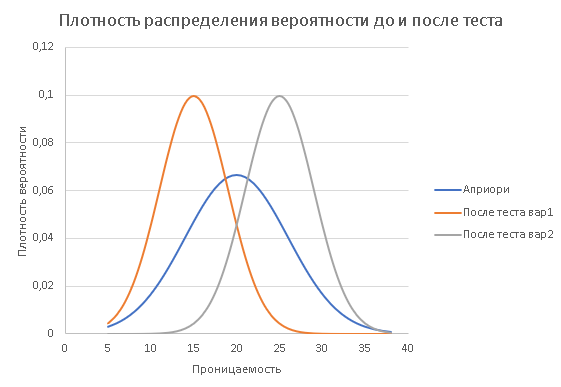
\includegraphics[width= 15cm]{pics_2/norm_distribution_ex1.png} 
	\label{fig:sample2}
	\caption{Иллюстрация к уточнению проницаемости в ходе исследований}
\end{figure}

Такой подход является явным упрощением. По приведённым ссылкам можно найти и другие подходы, где в частности предлагается учесть и менее явные последствия. Но его преимущество как раз в простоте. Он позволяет количественно оценить эффект от проведения исследований, соотнести его с затратами на проведение исследований и построить критерий принятия решений, который уже можно далее обсуждать и улучшать. 


Существует много подходов к построению критерия принятия решений о необходимости проведения исследований [ссылка на making good decisions]. Мы рассмотрим один из них, широко применяемый в различных областях деятельности, особенной в экономике и компьютерных науках - метод построения деревьев решений. \cite{AL_appl_patt_2007}

\section{Деревья решений для планирования исследований}

% translation from https://github.com/SilverDecisions/SilverDecisions/wiki/1.-Decision-tree-model
Последовательность и неопределенность присущи практическому принятию решений. Первое означает, что лица, принимающие решения, должны рассматривать многоступенчатые стратегии, охватывающие несколько действий, следующих друг за другом, а не только одно действие. Вторая означает, что отдача, получаемая лицами, принимающими решения, зависит не только от действий, но и от внешних событий ( состояний мира), которые часто могут быть восприняты как случайные. Действия и реакции обычно переплетаются, что еще больше усложняет картину. Деревья решений используются в качестве модели, помогающей обнаружить, понять и передать структуру таких проблем, связанных с принятием решений.

Ниже представлено простое дерево решений, созданное с помощью программы SilverDecisions (файл SilverDecisions, содержащий это дерево, можно запустить \href{http://silverdecisions.pl/SilverDecisions.html?LOAD_SD_TREE_JSON=https://raw.githubusercontent.com/gubkin-rienm/isp/master/data/decision_tree/simple_invest_decision.json}{здесь}).
\marginpar{
        ссылку там есть - надо сделать QR на нее
        }
%\urldef{\myurl}{http://silverdecisions.pl/SilverDecisions.html?LOAD_SD_TREE_JSON=https://raw.githubusercontent.com/gubkin-rienm/isp/master/data/decision_tree/simple_invest_decision.json}

\begin{figure}[h!]
	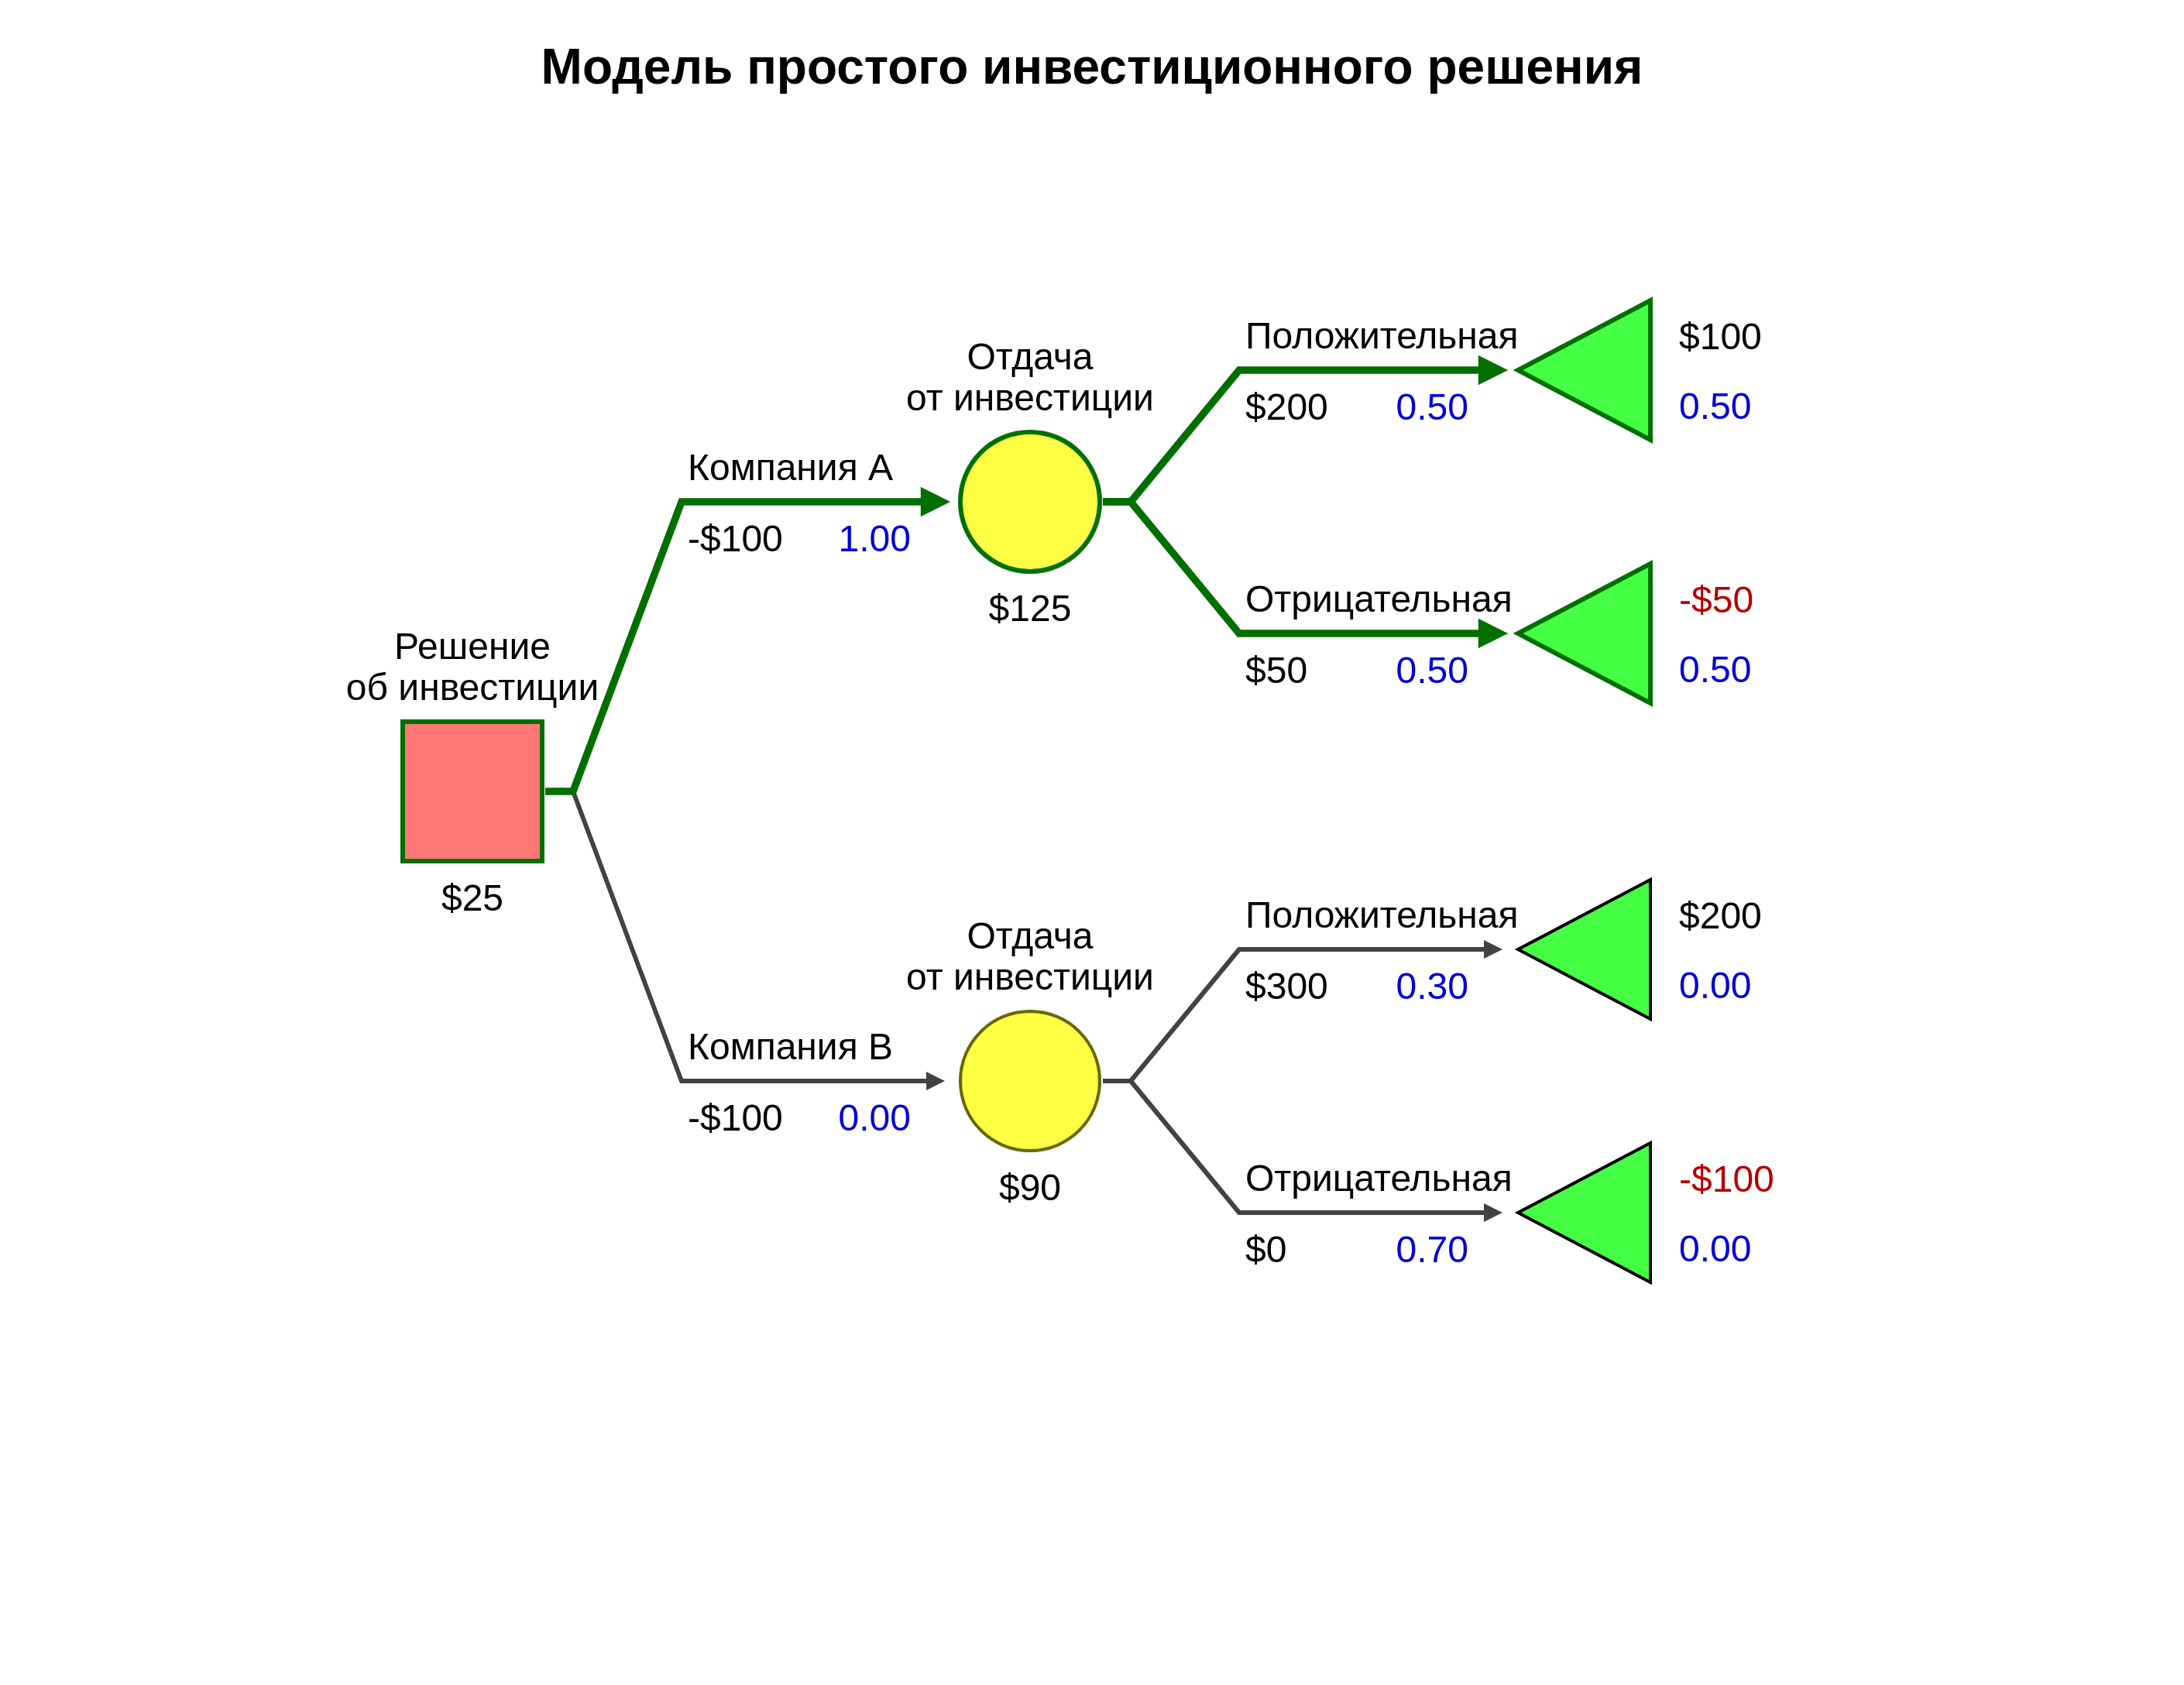
\includegraphics[width= 15cm]{pics/simple_decision_tree_1.png} 
	\label{fig:sample}
	\caption{Простое дерево решений}
\end{figure}

Модель дерева решений описывает и визуализирует последовательность принятия решения в условиях неопределенности на древовидной диаграмме. Это означает, что деревья решений могут быть полезны в таких задачах:
\begin{itemize}
    \item лицо, принимающее решение, выполняет несколько действий, следуя друг за другом,
    \item состояния мира могут различаться в зависимости от уже принятых решений,
    \item некоторые решения могут привести к более точным оценкам вероятности этих состояний.
\end{itemize}

На древовидной диаграмме представлены возможные решения, которые необходимо принять, независимые события, которые могут произойти, и результаты, связанные с комбинациями этих решений и событий. Необходимо определить два параметра: вероятности событий и их значения или стоимости. Первый параметр представляет вероятность получения определенного состояния мира. Поскольку возможные состояния мира в рамках одной реакции на самом деле являются конкурирующими событиями, сумма их вероятностей должна быть равна 1. 
Тогда значения или стоимости, выраженные в некоторой шкале, например в деньгах, означают платежи (изменение стоимости) как следствие решения или состояния мира. 
Это может быть как прибыль, так и убытки. Модель дерева решений включает еще одно понятие: EMV - ожидаемая значение или ожидаемая ценность (или ожидаемая полезность). Она вычисляется как вероятностно-взвешенное среднее значений для конкурирующих наборов решений и событий. Ожидаемое значение EMV показывает, сколько человек может заработать или потерять, принимая оптимальные решения (это означает такие решения, которые максимизируют прибыль и минимизируют убытки). Наконец, результат, связанный с решениями и событиями, представляет собой общее последствие набора решений и событий во всем процессе принятия решения. Он может быть истолкован как отдача лица, принимающего решение - результат как его решений, так и произошедших независимых событий.

Деревья решений с их простой для понимания структурой являются отличным инструментом для решения задач анализа. Они позволяют исследовать возможные результаты принятия решений и помогают выбирать между различными направлениями действий. Основной целью модели дерева решений является определение наилучшей возможной политики, которая представляет собой наибольшую отдачу или наименьший убыток.


Дерево решений строится по направленному графику слева направо, с набором узлов, которые разбиваются на три разрозненных множества:
\begin{itemize}
    \item узлы решения - типично представленные в виде квадратов,
    \item случайные узлы, представленные в виде кругов,
    \item терминальные узлы представлены в виде треугольников.
\end{itemize}

Крайняя левая вершина называется корневой вершиной и является первой вершиной принятия решения (первый красный квадрат слева - см. выше простую модель принятия инвестиционного решения - рисунок \ref{fig:sample} ). В узлах принятия решений выбирает именно тот, кто принимает решение, т.е. выбирает ровно одну из ветвей, выходящих из этого узла. Эти ветви представляют собой набор доступных альтернатив решения (действий). В случайном узле (желтые кружки - дерево образцов выше) каждая из вытекающих из него ребер - реакция - выбирается случайным образом с заданной вероятностью события. Терминальные узлы (синие треугольники на дереве выборки выше) представляют собой результат последовательности действий/реакций от корневого узла к данному конкретному терминальному узлу. Терминальный узел является конечной точкой: никакие решения не могут быть приняты, и никакие события не могут произойти после этого.

В приложении SilverDecisions вероятность событий и значения, связанные с этими событиями или решениями, определяются по краям. Ожидаемые значения, рассчитанные для каждого набора решений/событий, отображаются в каждом узле решения/шанса, а терминальные узлы показывают результаты и вероятности того, что событие окажется в указанном терминальном узле.

Обратите внимание, что каждое ребро совмещается с двумя узлами: левый, из которого выходит ребро, называется родительским узлом, а второй, находящийся справа, называется дочерним узлом. Поддерево - это еще один термин, связанный с деревьями решений - оно представляет собой ту часть дерева, которая начинается в любом дочернем узле, и каждый из них вместе с любыми потомками образует поддерево. Например, поддерево, уставившееся в корневой узел, представляет собой целое дерево.






\section{Задачи с примерами решения}

Деревья решений являются удобным инструментом для формализации процесса принятия решений. Они достаточно широко используются в нефтяной индустрии [привести ссылки на книгу и статьи]. 

Для построения деревьев решений можно использовать ручку, бумагу и калькулятор, так расчеты достаточно просты. Но удобнее использовать специализированные программные инструменты. Далее мы будем использовать сайт \url{http://silverdecisions.pl/} предоставляющий удобный, и что не менее важно, бесплатный и открытый программный комплекс для построения и анализа деревьев решений.

\subsection{Исследования на разведочной скважине}
    
    
Оцените стоит ли проводить комплекс исследований на разведочной скважине со следующими параметрами:
\begin{itemize}
    \item Стоимость 1 млн руб
    \item Ожидаемая информация – фильтрационные параметры пласта, уточнение строение пласта
    \item Вероятность успешности исследования (получения какой то информации) 70%
    \item Ожидается что исследование подтвердит увеличение запасов на 15% (60% что запасы увеличатся)
    \item Текущие извлекаемые запасы – 1 млн т. нефти, стоимость 1 т.нефти в запасах – 1 тыс. руб.
\end{itemize}     
Стоит ли проводить исследование? 

    
\subsection{КВД на добывающей скважине}

Оцените стоит ли проводить КВД на эксплуатационной скважине с дебитом 50 т/нефти, Рзаб = 50 атм, Рпл = 250 атм
\begin{itemize}
    \item Стоимость исследования 1 млн руб
    \item Длительность 1 неделя (скважина остановлена)
    \item Ожидаемая информация – фильтрационные параметры пласта, скин фактор
    \item Вероятность успешности исследования (получения какой то информации) 70%
    \item Ожидается что исследование подтвердит наличие положительного скин фактора
    \begin{itemize}
        \item S=0 с вероятностью 50%
        \item S=5 с вероятностью 40%
        \item S=15 с вероятностью 10%
    \end{itemize}
    \item Стоимость кислотной обработки снижающей скин в 2 раза 1 млн руб. Длительность эффекта 1 год
    \item Стоимость нефти 1 т = 10 тыс. руб.
\end{itemize}
Стоит ли проводить исследование? 

\subsection{Исследование фонтанирующей скважины}
Имеется фонтанирующая скважина. Дебит нефти 30 т/сут. Воды нет. Имеется водоносный пласт под продуктивным. Перемычка 10 м. Вероятность получения прорыва воды после ГРП 50 \%. При прорыве воды рост обводненности до 90 \% без увеличения дебита нефти. Без прорыва воды увеличение продуктивности в 3 раза. Стоимость ГРП 1 млн. руб.

Оценить что делать на скважине?

Ничего не делать
Сделать ГРП
Провести исследование и по его результатам ГРП
Стоимость исследования 100 т.р.

Вероятность выявления скважины где ГРП будет успешен 60%

\chapter{Исследования физико-химических свойств пластовых флюидов}

Здесь основные определения и теоретический минимум для последующих разделов. 
И набор мелких "коварных" задач для контроля знаний.
\section{Теория и определения}
\begin{itemize}
    \item Пластовые флюиды. Вода, нефть, газ.
    \item Модели флюидов. Модель нелетучей нефти. Композиционная модель. Основные предположения и отличия
    \item Параметры нефти для модели нелетучей нефти. Из зависимость от давления и температуры. 
    \item Параметры газа. z фактор. Коэффициент Джоуля Томсона для углеводородных газов. 
    \item Параметры воды и пара.
    
\end{itemize}
\section{Методы определения свойств флюидов}
Отбор глубинных проб, замеры на поверхности. Экспресс методы исследования.
\section{Задачи}
Расчеты с использованием Excel, Python, специализированное ПО
\begin{itemize}
    \item Зависимости параметров нефти воды и растворенного газа от давления и температуры (можно с использованием унифлок Excel)
    \item Построить график плотности воды при одновременно изменяющихся давлении и температуре
    \item Построить график зависимости доли свободного газа  от давления и температуры в потоке
    \item Оценить изменение температуры газа и ГЖС при изменении давления из за эффекта Джоуля Томсона
    \item Рассчитать изменение свойств воды и пара при нагреве.
    \item оценка газового фактора по данным замера расхода газа и нефти - учет растворенного в нефти газа на замерной с высоким давлением.

    % недавно было обнаружено что график достаточно странно выглядит :) 
    %\item Расчеты закона Дарси для трубы и простые задачи по линейному потоку в пласте. Определить перепад давления в трубе, оценить скорость движения жидкости и так далее.
\end{itemize}
    


\chapter{Барометрические исследования и расчет распределения давления в скважине и трубопроводах}

\section{Барометрические исследования и расчет распределения давления в скважине и трубопроводах}

Давление - ключевой параметр в системе пласт - скважина - скважинное оборудование. Перепад давления вызывает движение флюидов. Давлением можно управлять с помощью оборудования. Поэтому замеры давления и исследования построенные на контроле давления - ключевые для нефтедобычи.

Поскольку нефть и пластовые флюиды транспортируются по трубам - то изучение многофазного потока в трубах и скважинах занимает заметное место в управлении добычей. На моделировании этих процессов основан ряд методов исследования. 

В этом разделе посмотрим некоторые подходы к моделированию систем нефтедобычи и проведению исследований этих систем связанных с замерами давления.

\subsection{Теория}
\begin{itemize}
    \item Измерение давлений - датчики и принципы. Краткий обзор и ссылки. Принципы измерения давления, температурная компенсация, Приборы для измерения давления в эксплуатируемой скважине
    \item Связь давления и движения флюидов в трубах и скважине. Формула Дарси-Вейсбаха, уравнение Навье Стокса. Важность учета PVT при моделировании потоков
    \item Методы расчета распределения давления в потоке. Краткой обзор методов и программ. Примеры расчета.
    \item 
\end{itemize}

\subsection{Методы исследования с использованием измерений давления}
\begin{itemize}
    \item Забойное давление - ключевой параметр для контроля работы скважины. Методы контроля забойного давления - прямые измерения и косвенные оценки для различных типов скважин. Частота измерения забойного давления. Цели и задачи измерения забойного давления.
    \item Хранение результатов измерений давления. Шахматка, Техрежим, БСИ ЭЦН, корпоративные базы данных.
    \item Барометрия в работающей скважине
    \item Оценка параметров работы заглушенных скважин
\end{itemize}

\subsection{Задачи}

Задачи с использованием Excel и пакетов программ. 

\begin{itemize}
    \item Расчет распределения давления в скважине с использованием гидравлических корреляций. Построение кривой распределения давления в скважине.
    \item Расчет забойного давления по динамическому уровню в скважине с ЭЦН. Анализ отжима динамического уровня. 
    \item Оценка пластового давления в заглушенной скважине
\end{itemize}


\chapter{Термометрические исследования и расчет распределения температуры потока в скважине и трубопроводах}

\section{Термометрические исследования и расчет распределения температуры потока в скважине и трубопроводах}

\subsection{Теория}
\begin{itemize}
    \item Теория по замеру температуры в стволе скважины и в потоке
    \item Принципы измерения температуры и датчики температуры
\end{itemize}


\subsection{Методы исследования с использованием измерений температуры}

\begin{itemize}
    \item Термометрия в стволе скважины. Расчет температуры на устье. Выявление зон опасных для отложения парафинов гидратов
    
    \item Термометрия в продуктивном интервале 
    
    \item Термометрия в газлифтной скважине для анализа работы газлифтных клапанов
    
    \item Температурный режим работы ЭЦН. Предотвращение отказов ЭЦН на основе замеров температуры
\end{itemize}

\subsection{Задачи}

Задачи с использованием Excel и пакетов программ. 

\begin{itemize}
    \item Расчет распределения температуры в скважине с учетом притока разных флюидов в скважине
    \item Калориметрическое смешивание
    \item Расчет распределения температуры в газлифтной скважине
    \item Расчет температурного режима работы ЭЦН
    \item Расчет температуры и отложение гидратов
    
\end{itemize}


\chapter{Дебитометрия в скважине и на поверхности. Принципы замера дебита и виртуальный расходомер.}

% хороший раздел - но тут сложно придумать хорошие задачи 
% на практике дебитам либо верим и используем, либо не верим
% дебитограммы никто нынче особо не смотрит 
% хотя можно сделать блок по построению дебитограмм из синтетических данных
% и примеры с интерпретацией соответственно 
\section{Теория}
\begin{itemize}
    \item Принципы измерения дебита (расхода). Оборудования для измерения дебита на поверхности и в скважине
    \item Замер обводненности и газового фактора продукции
    \item Замеры количества механических примесей
    \item Профили притока к скважине. Замер профиля притока с использованием скважинного оборудования
\end{itemize}

\section{Задачи}

\begin{itemize}
    \item Оценка дебита по закону Бернулли - на гидравлическом сужении. Оценка дебита по характеристике потока через штуцер
    \item Оценка обводненности по данным замером плотности флюидов и плотности смеси
    \item Оценка газового фактора по данным эксплуатации скважины - перепад давления в скважине и на штуцере
    \item Оценка газового фактора по данным отжима динамического уровня
    \item Расчет профиля изменения давления и профиля притока в горизонтальной скважине (учет по плотности притока и диаметру ствола скважины)
    
\end{itemize}
%\section{Выявление нарушений герметичности ствола скважины}
    


\section{Теория температура}

давления и температуру лучше совместить в один раздел, чтобы было меньше глав



\chapter{Список тем для самостоятельно изучения (рефераты)}

\end{document}
